\documentclass[11pt,oneside]{article}
\usepackage[T1]{fontenc}
\usepackage[utf8]{inputenc}
% \usepackage{lmodern}
%\usepackage[adobe-utopia,uppercase=upright,greeklowercase=upright]{mathdesign}
\usepackage[adobe-utopia]{mathdesign}
%\usepackage{minionpro}
% \usepackage{pifont}
% \usepackage{amssymb}
\usepackage{amsmath}
\usepackage[francais]{babel}
% \usepackage[francais]{varioref}
\usepackage[dvips]{graphicx}

\usepackage{framed}
\usepackage[normalem]{ulem}
\usepackage{fancyhdr}
\usepackage{titlesec}
\usepackage{vmargin}
\usepackage{longtable}

\usepackage{ifthen}


%\usepackage{epsfig}
\usepackage{subfig}

\usepackage{multirow}
\usepackage{multicol} % Portions de texte en colonnes
\usepackage{flafter}%floatants après la référence



\usepackage{color}
\usepackage{colortbl}


\definecolor{gris25}{gray}{0.75}
\definecolor{bleu}{RGB}{18,33,98}
\definecolor{bleuf}{RGB}{42,94,171}
\definecolor{bleuc}{RGB}{231,239,247}
\definecolor{rougef}{RGB}{185,18,27}
\definecolor{rougec}{RGB}{255,230,231}
\definecolor{vertf}{RGB}{103,126,82}
\definecolor{vertc}{RGB}{220,255,191}

\newenvironment{rem}[1][\hsize]%
{%
    \def\FrameCommand
    {%
\rotatebox{90}{\textit{\textsf{Remarque}}} 
        {\color{bleuf}\vrule width 3pt}%
        \hspace{0pt}%must no space.
        \fboxsep=\FrameSep\colorbox{bleuc}%
    }%
    \MakeFramed{\hsize#1\advance\hsize-\width\FrameRestore}%
}%
{\endMakeFramed}%


\newenvironment{savoir}[1][\hsize]%
{%
    \def\FrameCommand
    {%
\rotatebox{90}{\textit{\textsf{Savoir}}} 
        {\color{bleuf}\vrule width 3pt}%
        \hspace{0pt}%must no space.
        \fboxsep=\FrameSep\colorbox{bleuc}%
    }%
    \MakeFramed{\hsize#1\advance\hsize-\width\FrameRestore}%
}%
{\endMakeFramed}%

\newenvironment{prob}[1][\hsize]%
{%
    \def\FrameCommand%
    {%
\rotatebox{90}{\textit{\textsf{ Problématique}}} 
        {\color{rougef}\vrule width 3pt}%
        \hspace{0pt}%must no space.
        \fboxsep=\FrameSep\colorbox{rougec}%
    }%
    \MakeFramed{\hsize#1\advance\hsize-\width\FrameRestore}%
}%
{\endMakeFramed}%

\newenvironment{obj}[1][\hsize]%
{%
    \def\FrameCommand%
    {%
\rotatebox{90}{\textit{\textsf{ $\;$}}} 
        {\color{rougef}\vrule width 3pt}%
        \hspace{0pt}%must no space.
        \fboxsep=\FrameSep\colorbox{rougec}%
    }%
    \MakeFramed{\hsize#1\advance\hsize-\width\FrameRestore}%
}%
{\endMakeFramed}%

\newenvironment{defi}[1][\hsize]%
{%
    \def\FrameCommand%
    {%
\rotatebox{90}{\textit{\textsf{Définition\\}}} 
        {\color{bleuf}\vrule width 3pt}%
        \hspace{0pt}%must no space.
        \fboxsep=\FrameSep\colorbox{bleuc}%
    }%
    \MakeFramed{\hsize#1\advance\hsize-\width\FrameRestore}%
}%
{\endMakeFramed}%


\newenvironment{hypo}[1][\hsize]%
{%
    \def\FrameCommand%
    {%
\rotatebox{90}{\textit{\textsf{Hypothèse\\}}} 
        {\color{bleuf}\vrule width 3pt}%
        \hspace{0pt}%must no space.
        \fboxsep=\FrameSep\colorbox{bleuc}%
    }%
    \MakeFramed{\hsize#1\advance\hsize-\width\FrameRestore}%
}%
{\endMakeFramed}%


\newenvironment{prop}[1][\hsize]%
{%
    \def\FrameCommand%
    {%
\rotatebox{90}{\textit{\textsf{Propriété\\}}} 
        {\color{bleuf}\vrule width 3pt}%
        \hspace{0pt}%must no space.
        \fboxsep=\FrameSep\colorbox{bleuc}%
    }%
    \MakeFramed{\hsize#1\advance\hsize-\width\FrameRestore}%
}%
{\endMakeFramed}%

\newenvironment{props}[1][\hsize]%
{%
    \def\FrameCommand%
    {%
\rotatebox{90}{\textit{\textsf{Propriétés\\}}} 
        {\color{bleuf}\vrule width 3pt}%
        \hspace{0pt}%must no space.
        \fboxsep=\FrameSep\colorbox{bleuc}%
    }%
    \MakeFramed{\hsize#1\advance\hsize-\width\FrameRestore}%
}%
{\endMakeFramed}%

\newenvironment{exemple}[1][\hsize]%
{%
    \def\FrameCommand%
    {%
\rotatebox{90}{\textit{\textsf{Exemple\\}}} 
        {\color{vertf}\vrule width 3pt}%
        \hspace{0pt}%must no space.
        \fboxsep=\FrameSep\colorbox{vertc}%
    }%
    \MakeFramed{\hsize#1\advance\hsize-\width\FrameRestore}%
}%
{\endMakeFramed}%

\newenvironment{resultat}[1][\hsize]%
{%
    \def\FrameCommand%
    {%
\rotatebox{90}{\textit{\textsf{Résultat\\}}} 
        {\color{rougef}\vrule width 3pt}%
        \hspace{0pt}%must no space.
        \fboxsep=\FrameSep\colorbox{rougec}%
    }%
    \MakeFramed{\hsize#1\advance\hsize-\width\FrameRestore}%
}%
{\endMakeFramed}%

\newenvironment{methode}[1][\hsize]%
{%
    \def\FrameCommand%
    {%
\rotatebox{90}{\textit{\textsf{Méthode\\}}} 
        {\color{rougef}\vrule width 3pt}%
        \hspace{0pt}%must no space.
        \fboxsep=\FrameSep\colorbox{rougec}%
    }%
    \MakeFramed{\hsize#1\advance\hsize-\width\FrameRestore}%
}%
{\endMakeFramed}%

\newenvironment{theo}[1][\hsize]%
{%
    \def\FrameCommand%
    {%
\rotatebox{90}{\textit{\textsf{Théorème\\}}} 
        {\color{rougef}\vrule width 3pt}%
        \hspace{0pt}%must no space.
        \fboxsep=\FrameSep\colorbox{rougec}%
    }%
    \MakeFramed{\hsize#1\advance\hsize-\width\FrameRestore}%
}%
{\endMakeFramed}%

\newenvironment{warn}[1][\hsize]%
{%
    \def\FrameCommand%
    {%
\rotatebox{90}{\textit{\textsf{Attention\\}}} 
        {\color{rougef}\vrule width 3pt}%
        \hspace{0pt}%must no space.
        \fboxsep=\FrameSep\colorbox{rougec}%
    }%
    \MakeFramed{\hsize#1\advance\hsize-\width\FrameRestore}%
}%
{\endMakeFramed}%

% \usepackage{pstricks}
%\usepackage{minitoc}
% \setcounter{minitocdepth}{4}

\setcounter{tocdepth}{2}

% \mtcselectlanguage{french} 

%\usepackage{draftcopy}% "Brouillon"
% \usepackage{floatflt}
\usepackage{psfrag}
%\usepackage{listings} % Permet d'insérer du code de programmation
\renewcommand{\baselinestretch}{1.2}

% Changer la numérotation des figures :
% ------------------------------------
% \makeatletter
% \renewcommand{\thefigure}{\ifnum \c@section>\z@ \thesection.\fi
%  \@arabic\c@figure}
% \@addtoreset{figure}{section}
% \makeatother
 


%%%%%%%%%%%%
% Définition des vecteurs %
%%%%%%%%%%%%
 \newcommand{\vect}[1]{\overrightarrow{#1}}

%%%%%%%%%%%%
% Définition des torseusr %
%%%%%%%%%%%%

 \newcommand{\torseur}[1]{%
\left\{{#1}\right\}
}

\newcommand{\torseurcin}[3]{%
\left\{\mathcal{#1} \left(#2/#3 \right) \right\}
}

\newcommand{\torseurstat}[3]{%
\left\{\mathcal{#1} \left(#2\rightarrow #3 \right) \right\}
}

 \newcommand{\torseurc}[8]{%
%\left\{#1 \right\}=
\left\{
{#1}
\right\}
 = 
\left\{%
\begin{array}{cc}%
{#2} & {#5}\\%
{#3} & {#6}\\%
{#4} & {#7}\\%
\end{array}%
\right\}_{#8}%
}

 \newcommand{\torseurcol}[7]{
\left\{%
\begin{array}{cc}%
{#1} & {#4}\\%
{#2} & {#5}\\%
{#3} & {#6}\\%
\end{array}%
\right\}_{#7}%
}

 \newcommand{\torseurl}[3]{%
%\left\{\mathcal{#1}\right\}_{#2}=%
\left\{%
\begin{array}{l}%
{#1} \\%
{#2} %
\end{array}%
\right\}_{#3}%
}

 \newcommand{\vectv}[3]{%
\vect{V\left( {#1} \in {#2}/{#3}\right)}
}


\newcommand{\vectf}[2]{%
\vect{R\left( {#1} \rightarrow {#2}\right)}
}

\newcommand{\vectm}[3]{%
\vect{\mathcal{M}\left( {#1}, {#2} \rightarrow {#3}\right)}
}


 \newcommand{\vectg}[3]{%
\vect{\Gamma \left( {#1} \in {#2}/{#3}\right)}
}

 \newcommand{\vecto}[2]{%
\vect{\Omega\left( {#1}/{#2}\right)}
}
% }$$\left\{\mathcal{#1} \right\}_{#2} =%
% \left\{%
% \begin{array}{c}%
%  #3 \\%
%  #4 %
% \end{array}%
% \right\}_{#5}}

%  ------------------------------------------
% | Modification du formatage des sections : | 
%  ------------------------------------------

% Grands titres :
% ---------------

\newcommand{\titre}[1]{%
\begin{center}
      \bigskip
      \rule{\textwidth}{1pt}
      \par\vspace{0.1cm}
      
      \textbf{\large #1}
      \par\rule{\textwidth}{1pt}
    \end{center}
    \bigskip
  }

% Supprime le numéro du chapitre dans la numérotation des sections:
% -----------------------------------------------------------------
\makeatletter
\renewcommand{\thesection}{\@arabic\c@section}
\makeatother


% \titleformat{\chapter}[display]
% {\normalfont\Large\filcenter}
% {}
% {1pc}
% {\titlerule[1pt]
%   \vspace{1pc}%
%   \Huge}[\vspace{1ex}%
% \titlerule]


%%%% Chapitres Comme PY Pechard %%%%%%%%%
% numéro du chapitre
\DeclareFixedFont{\chapnumfont}{OT1}{phv}{b}{n}{80pt}
% pour le mot « Chapitre »
\DeclareFixedFont{\chapchapfont}{OT1}{phv}{m}{it}{40pt}
% pour le titre
\DeclareFixedFont{\chaptitfont}{T1}{phv}{b}{n}{25pt}

\definecolor{gris}{gray}{0.75}
\titleformat{\chapter}[display]%
	{\sffamily}%
	{\filleft\chapchapfont\color{gris}\chaptertitlename\
	\\
	\vspace{12pt}
	\chapnumfont\thechapter}%
	{16pt}%
	{\filleft\chaptitfont}%
	[\vspace{6pt}\titlerule\titlerule\titlerule]

%%%%  Fin Chapitres Comme PY Pechard %%%%%%%%%


% Section, subsection, subsubsection sans serifs :
% % ----------------------------------------------

% \makeatletter
% \renewcommand{\section}{\@startsection{section}{0}{0mm}%
% {\baselineskip}{.3\baselineskip}%
% {\normalfont\sffamily\Large\textbf}}%
% \makeatother

\makeatletter
\renewcommand{\@seccntformat}[1]{{\textcolor{bleu}{\csname
the#1\endcsname}\hspace{0.5em}}}
\makeatother

\makeatletter
\renewcommand{\section}{\@startsection{section}{1}{\z@}%
                       {-4ex \@plus -1ex \@minus -.4ex}%
                       {1ex \@plus.2ex }%
                       {\normalfont\Large\sffamily\bfseries}}%
\makeatother
 
\makeatletter
\renewcommand{\subsection}{\@startsection {subsection}{2}{\z@}
                          {-3ex \@plus -0.1ex \@minus -.4ex}%
                          {0.5ex \@plus.2ex }%
                          {\normalfont\large\sffamily\bfseries}}
\makeatother
 
\makeatletter
\renewcommand{\subsubsection}{\@startsection {subsubsection}{3}{\z@}
                          {-2ex \@plus -0.1ex \@minus -.2ex}%
                          {0.2ex \@plus.2ex }%
                          {\normalfont\large\sffamily\bfseries}}
\makeatother
 
\makeatletter             
\renewcommand{\paragraph}{\@startsection{paragraph}{4}{\z@}%
                                    {-2ex \@plus-.2ex \@minus .2ex}%
                                    {0.1ex}%               
{\normalfont\sffamily\bfseries}}
\makeatother
 
\makeatletter
\renewcommand{\subparagraph}{\@startsection{subparagraph}{5}{\z@}%
                                       {-2ex \@plus-.1ex \@minus .2ex}%
                                       {0.1ex}%
				    {\normalfont\normalsize\sffamily\bfseries}}
\makeatletter
% \makeatletter
% \renewcommand{\subsection}{\@startsection{subsection}{1}{2mm}%
% {\baselineskip}{.3\baselineskip}%
% {\normalfont\sffamily\large\textbf}}%
% \makeatother
% 
% \makeatletter
% \renewcommand{\subsubsection}{\@startsection{subsubsection}{2}{4mm}%
% {\baselineskip}{.15\baselineskip}%
% {\normalfont\sffamily\large\textbf}}%
% \makeatother
% 
% \makeatletter
% \renewcommand{\paragraph}{\@startsection{paragraph}{3}{6mm}%
% {\baselineskip}{.15\baselineskip}%
% {\normalfont\sffamily\large\textbf}}%
% \makeatother
 
\setcounter{secnumdepth}{4}


%  --------
% | Marges |
%  --------


% \setmarginsrb{2.5cm}{1.5cm}{2.5cm}{2cm}{1cm}{1cm}{1cm}{1cm}
\setmarginsrb{1.5cm}{1cm}{1cm}{1.5cm}{1cm}{1cm}{1cm}{1cm}

% Changer les marges localement :
% -----------------------------
\newenvironment{changemargin}[2]{\begin{list}{}{%
\setlength{\topsep}{0pt}%
\setlength{\leftmargin}{0pt}%
\setlength{\rightmargin}{0pt}%
\setlength{\listparindent}{\parindent}%
\setlength{\itemindent}{\parindent}%
\setlength{\parsep}{0pt plus 1pt}%
\addtolength{\leftmargin}{#1}%
\addtolength{\rightmargin}{#2}%
}\item }{\end{list}}



\usepackage{pst-solides3d}
\usepackage{titletoc}
\titlecontents{chapter}[+3pc]
  {\addvspace{10pt}\sffamily\bfseries}
{\contentslabel[{\pscirclebox[fillstyle=solid,fillcolor=gray!25,
linecolor=gray!25,framesep=4pt]{\textcolor{white}{\thecontentslabel}}}]{2.5pc}}
  {}
  {\dotfill \normalfont\thecontentspage\ }

\titlecontents{section}[3pc]
  {\addvspace{2pt}\sffamily}
  {\contentslabel[\thecontentslabel]{1.8pc}}
  {}
  {\dotfill \normalfont\thecontentspage\ }

\titlecontents{subsection}[5pc]
  {\addvspace{2pt}\sffamily}
  {\contentslabel[\thecontentslabel]{1.8pc}}
  {}
  {\dotfill \normalfont\thecontentspage\ }

\titlecontents{subsubsection}[8pc]
  {\addvspace{2pt}\sffamily}
  {\contentslabel[\thecontentslabel]{3pc}}
  {}
  {\dotfill \normalfont\thecontentspage\ }
%{\;\titlerule\;\normalfont\thecontentspage\ }

\titlecontents{paragraph}[9pc]
  {\addvspace{2pt}\sffamily}
  {\contentslabel[\thecontentslabel]{3.5pc}}
  {}
  {\dotfill \normalfont\thecontentspage\ }




\usepackage[%
    pdftitle={DM5 - Cinématique},
    pdfauthor={Xavier Pessoles},
    colorlinks=true,
    linkcolor=blue,
    citecolor=magenta]{hyperref}

\usepackage{schemabloc}

% \makeatletter \let\ps@plain\ps@empty \makeatother
%% DEBUT DU DOCUMENT
%% =================
\sloppy
\hyphenpenalty 10000



\colorlet{shadecolor}{orange!15}

\begin{document}


\newboolean{prof}
\setboolean{prof}{true}
%------------- En tetes et Pieds de Pages ------------
\pagestyle{fancy}
\renewcommand{\headrulewidth}{0pt}

\fancyhead{}
\fancyhead[L]{%
\begin{minipage}[c]{1.6cm}
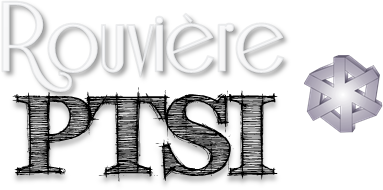
\includegraphics[width=2cm]{png/logo_ptsi.png}%
\end{minipage}
\rule{2cm}{.5pt}
}

\fancyhead[C]{\rule{11cm}{.5pt}}

\fancyhead[R]{%
\begin{minipage}[c]{3cm}
\begin{flushright}
\footnotesize{\textit{\textsf{Sciences Industrielles\\ de l'Ingénieur}}}%
\end{flushright}
\end{minipage}
}

\renewcommand{\footrulewidth}{0.2pt}

\fancyfoot[C]{\footnotesize{\bfseries \thepage}}
\fancyfoot[L]{\footnotesize{2012 -- 2013} \\ X. \textsc{Pessoles}}
\ifthenelse{\boolean{prof}}{%
\fancyfoot[R]{\footnotesize{DM 7}}
}{%
\fancyfoot[R]{\footnotesize{DM 6}}%-- CI 3 : Statique \& CI 6 : PPM}}
}


%\begin{center}
%\textit{Centre d'intérêt}
%\end{center}

\begin{center}
 \Large\textsc{Devoir Maison 7}
\end{center}

\begin{center}
 \large\textsc{Éléments de corrigé} 
\end{center}


\vspace{0.5cm}


\noindent\rule{\linewidth}{.2pt}
\begin{center}
 %\large\textbf{CI 4} \textit{Conception des mécanismes}

 \large\textbf{CI 5} \textit{Communication technique : Schémas et géométrie des pièces, architecture des systèmes pluritechniques}
\end{center}
\noindent\rule{\linewidth}{.2pt}


\vspace{0.5cm}




\noindent\rule{\linewidth}{.2pt}
\begin{center}
 \LARGE\textbf{\textsc{Boîte de transfert de 4x4}}
\end{center}
\noindent\rule{\linewidth}{.2pt}



\section{Étude préliminaire -- Analyse du besoin}

\paragraph{}
\textit{Déterminer l'angle de rotation de la roue gauche $\alpha_G$ du véhicule en fonction de $\alpha_D$, de l'empattement $e$ et de la voie $v$. L'empattement $e$ est la distance $DC$ entre les essieux avant et arrière. La voie $v$ est la distance $DG$ entre le centre des deux roues.}

On connait la direction du vecteur vitesse de $\vectv{M}{1}{sol}$ et de $\vectv{D}{1}{sol}$. On peut donc écrire le CIR du mouvement de 1 par rapport au sol. Pour cela, on trace les perpendiculaires aux deux vecteurs vitesse. 

Connaissant le CIR, on sait que $\vectv{G}{1}{sol}$ sera perpendiculaire à la droite $(IC)$. On peut donc déduire la direction de la roue gauche. 

\begin{center}
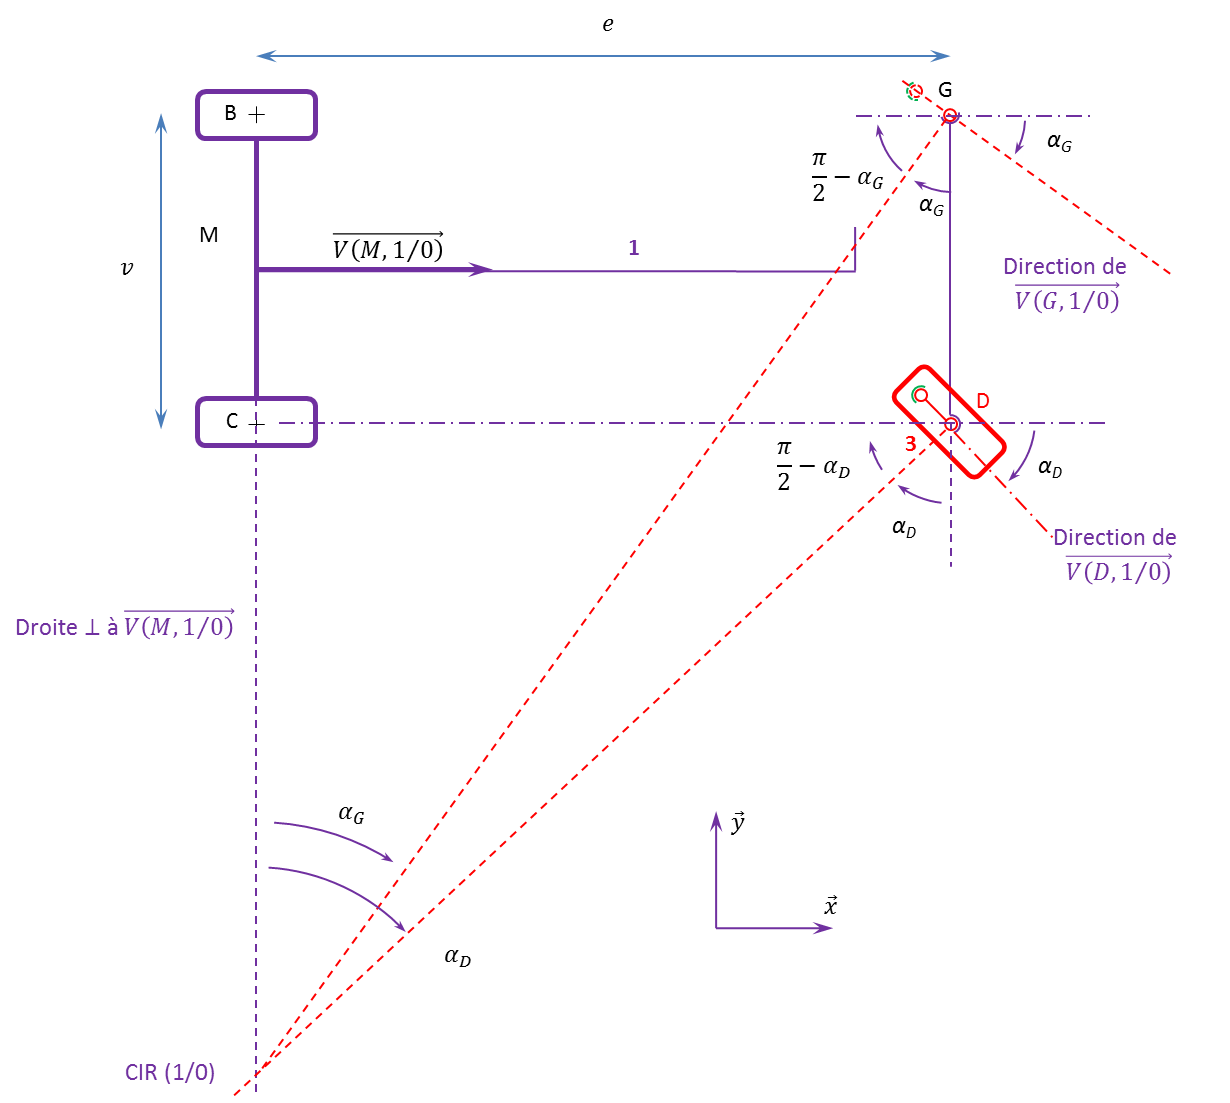
\includegraphics[width=.8\textwidth]{png/angle_roue}
\end{center}

D'une part, dans le triangle $CDI$ rectangle en $C$, on a :
$$
\tan\alpha_D = \dfrac{e}{CI} \Longleftrightarrow CI = \dfrac{e}{\tan\alpha_D}
$$

D'une part, dans le triangle $BGI$ rectangle en $B$, on a :
$$
\tan\alpha_G = \dfrac{e}{CI+v}
$$

En conséquence, 
$$
\tan\alpha_G = \dfrac{e}{\dfrac{e}{\tan\alpha_D}+v}=\dfrac{e\tan\alpha_D}{e+v\tan\alpha_D}
$$


\paragraph{}
\textit{Proposer un schéma cinématique minimal, à main levée, permettant de prendre en compte que les deux roues ne tournent pas du même angle lors d'un virage. }

Sans les biellettes supplémentaires,certaines roues déraperaient.

\paragraph{}
\textit{On donne $||\vectv{M}{1}{sol}||=30\; km/h$. L'angle de rotation de la roue droite est de $45\degres$. Déterminer graphiquement, sur le schéma en fin de document, la vitesse aux points $B$, $C$, $D$ et $G$. Que peut-on en conclure ?}

\begin{center}
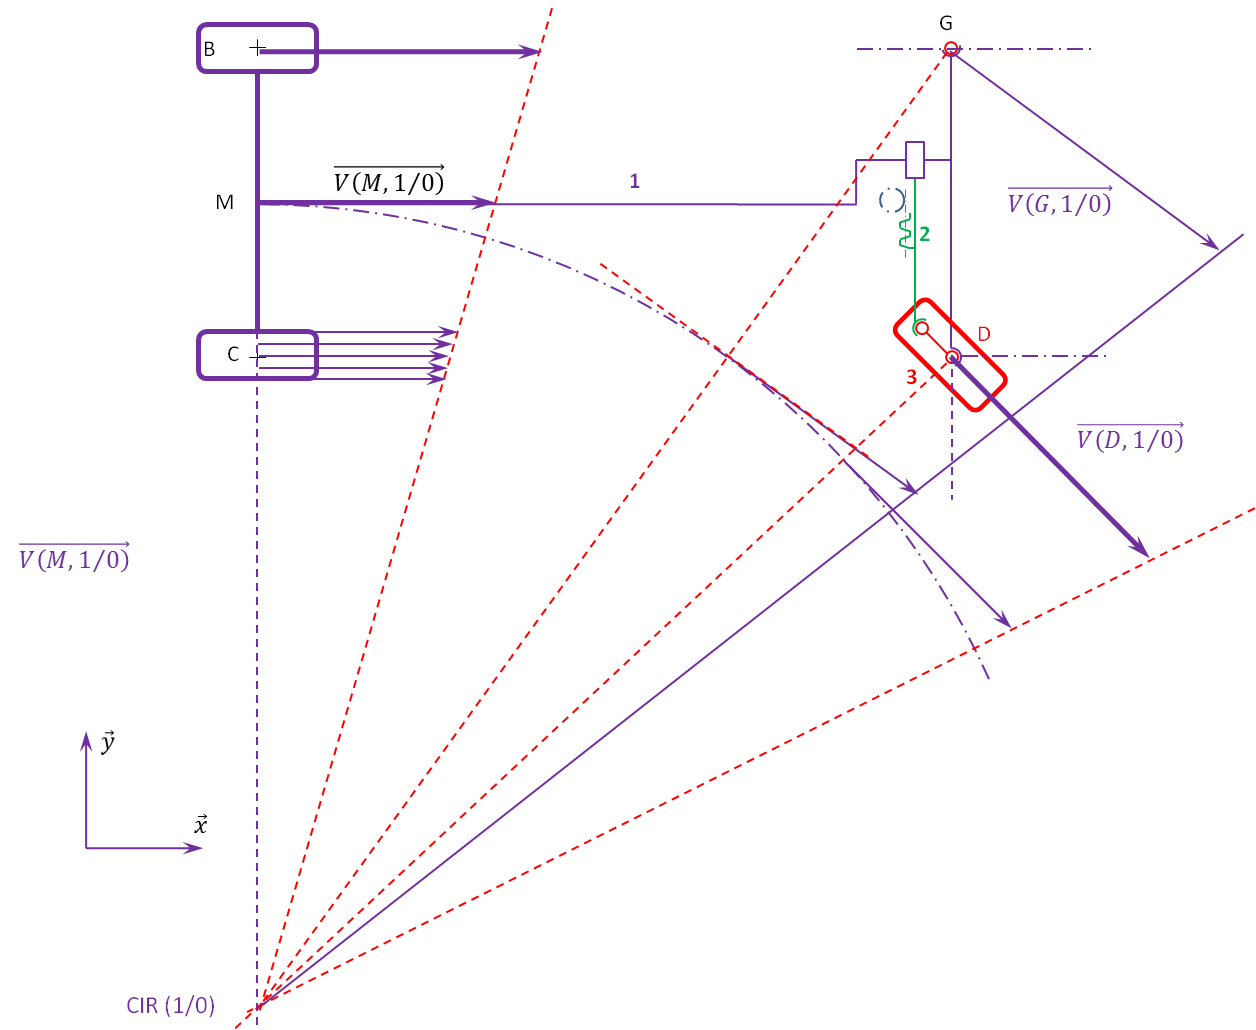
\includegraphics[width=.9\textwidth]{png/cin_graph}
\end{center}

Après étude graphique, on a :
\begin{itemize}
\item $||\vectv{B}{1}{sol}||= 36\; km/h$;
\item $||\vectv{C}{1}{sol}||= 24\; km/h$;
\item $||\vectv{D}{1}{sol}||= 36\; km/h$;
\item $||\vectv{G}{1}{sol}||= 42\; km/h$.
\end{itemize}


On conclut donc que dans un virage, les 4 roues n'ont pas la même vitesse. Sur un véhicule classique à traction, les roues arrières sont chacune montées sur les essieux par deux liaisons pivots indépendantes. 

Les roues avant sont liées à la boîte de vitesse. Si les deux roues étaient liées directement à la boîte de vitesse, la distance à parcourir par les deux roues seraient différentes lors des virages. 

Pour permettre aux roues de tourner à des vitesses différentes lors des virages, les véhicules sont équipés d'un différentiel en sortie de la boîte de vitesse. 

\paragraph{}
\textit{Tracer le champ des vecteurs vitesses sur une largeur de pneu lors d'un virage. Que peut-on en conclure ?}

Lors d'un virage, théoriquement, le champ des vecteurs vitesses n'est pas uniforme sur une largeur de pneu. Or, la liaison entre la roue et le châssis impose que le champ des vecteurs vitesses soit uniforme sur une largeur de pneu. En conséquence, le différentiel de vitesse nécessaire se traduit par un dérapage du pneu et donc une usure irrégulière.

\paragraph{}
\textit{En utilisant une bête à cornes, dire à quel besoin devra répondre la boîte de transfert du 4x4.}


\section{Boîte de transfert}

\subsection{Fonctionnement}

\subsection{Étude technologique}

\paragraph{}
\textit{D'après vous, comment est assurée la lubrification du système ? Comment est assurée la vidange ? Comment est assurée l'étanchéité vis-à-vis du milieu extérieur. }

La lubrification par barbotage des pignons dans un bain d'huile. La vidange a lieu grâce au bouchon indiqué "c". L'étanchéité dynamique du système est assuré grâce à des joints à lèvre. 

\paragraph{}
\textit{Citer les 4 différentes technologies de roulements présentes dans la boîte de transfert. Indiquer leurs particularités et leurs cas d'utilisation.}

Les roulements à billes à contact radial permettent de supporter des charges radiales et axiales. 

Les roulements à rouleaux cylindriques permettent de supporter des charges radiales importantes à des fréquences de rotations importantes. Ils ne supportent aucune charge axiale. Ils ont la particularité d'avoir une bague séparable.

Les roulements à aiguilles permettent de supporter des charges radiales et aucune charge axiale. Ils ont la particularité d'avoir un très faible encombrement. La plupart du temps, on peut noter l'absence de bagues intérieures et extérieures. Dans ce cas, les aiguilles roulent directement sur l'arbre et le moyeu. Il est donc nécessaire que ceux-ci aient une dureté importante (supérieure à $57 HRc$).

Les butées à billes (20) permettent de supporter des charges axiales importantes à de faibles fréquences de rotation. Elles ne permettent pas de guider l'arbre en rotation. Pour cela d'autres roulements sont nécessaires.  

\paragraph{}
\textit{On dénote un jeu entre la bague extérieure du roulement \textbf{32} et le flasque \textbf{30} ainsi que la carter \textbf{33}. Quel est son but ?}

Les deux roulements à rouleaux cylindriques permettent d'encaisser les efforts radiaux. Ce roulement à billes est présent pour encaisser la totalité des efforts axiaux. Il n'est donc pas nécessaire de l'ajuster sur la bague extérieure. 

\paragraph{}
\textit{Proposer un matériau pour l'arbre \textbf{6}. Comment a-t-il été fabriqué ?}

Cet arbre transmet la totalité de la puissance mécanique du véhicule (au rendement près). Il est donc fortement contraint. En conséquence, on choisit un acier ($25\; Cr\; Mo\; 4$ par exemple). 

Les procédés suivant ont pu être utilisés pour la fabrication de cet arbre : 
\begin{itemize}
\item laminage et découpe d'un cylindre;
\item forgeage à chaud;
\item tournage des portées de roulements et du filetage, des chanfreins;
\item fraisage de la rainure de clavette (fraise 2 tailles);
\item taillage de la roue dentée à l'outil pignon (ou crémaillère) (mortaisage);
\item traitements thermiques;
\item finition des surfaces fonctionnelles.
\end{itemize}


\paragraph{}
\textit{Un palier lisse est présent entre l'arbre \textbf{9} et la pièce \textbf{25}. Quel est son but ? Proposer un matériau ? Comment a-t-il été fabriqué ?}

Le but de ce palier lisse (ou coussinet) est de participer à la réalisation d'une liaison pivot. Il est en contact direct avec les pièces en mouvement. Le matériau couramment utilisé pour ce type de pièce est le bronze ($Cu \; Sn 8$). 

Ces coussinets sont frittés : du bronze en poudre est chauffé dans un moule. En chauffant, les grains se soudent entre eux entrainant la cohésion du matériau. Ils peuvent ensuite être plongés dans un bain d'huile pour leur conférer (en plus des propriété tribologique du bronze) une capacité à être auto lubrifiés. 

\subsection{Étude cinématique}

\paragraph{}
\textit{Identifiez les différentes classes d'ensemble cinématique en coloriant le dessin d'ensemble. On précise que les pièces \textbf{10} (couronne à denture intérieure), \textbf{11}  (pignon - satellite), \textbf{9} (pignon - planétaire) et \textbf{25} (porte-satellite) forment un train épicycloïdal\footnote{Seules les pièces principales des classes d'équivalences cinématiques sont citées.}.}


\paragraph{}
\textit{Quelle pièce permet le passage de la vitesse "route" à la vitesse 4x4" via le levier \textbf{V2} ? Quel est le mouvement de cette pièce ? Comment est-elle mise en mouvement ? Expliquer comment elle permet de sélectionner chacune des deux vitesses. Vous pourrez éventuellement vous aider de schémas.}

Le crabot \textbf{2} et l'arbre venant de la boîte de vitesse \textbf{4} sont en liaison glissière. Cette liaison est assurée par des cannelures. La translation du crabot est assuré par le levier \textbf{V2} (appelé aussi fourchette).

Lorsque le crabot est en position centrale, le véhicule est au point neutre. Dans ces conditions, les pignons \textbf{1} et \textbf{3} sont en liaison pivot par rapport à l'arbre \textbf{4} relié à la boîte de vitesse. Si cet arbre tourne, aucun couple est transmis. 

Lorsque le crabot est basculé vers la gauche, les cannelures de ce dernier s'engagent dans les cannelures du pignon. La position du crabot est verrouillée par l'intermédiaire de la bille venant se loger dans un perçage prévu à cet effet. Le crabotage permet de solidariser le pignon et l'arbre \textbf{4}. Le couple peut alors être transmis à l'arbre \textbf{6} via le pignon \textbf{5}.

\paragraph{}
\textit{Quelle influence a le levier \textbf{D} sur le fonctionnement de la boîte de transfert ?}

Ce levier permet de solidariser l'arbre de l'essieu avant avec le porte satellite du train épicycloïdal. Le différentiel est ainsi désactivé. 

\paragraph{}
\textit{En vous aidant des croquis présents sur le dessin d'ensemble, tracer le schéma cinématique minimal de la boîte de transfert. Vous pourrez utiliser le schéma cinématique du train épicycloïdal donné en fin de document en l'adaptant à notre cas.}

\begin{center}
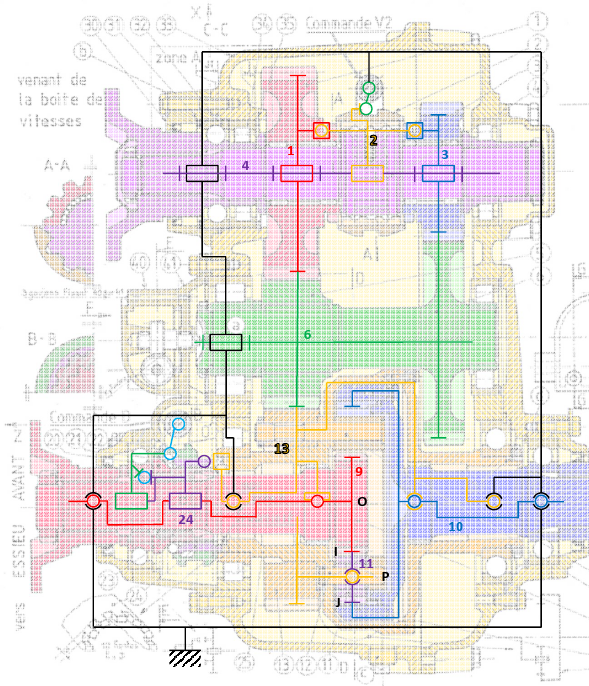
\includegraphics[width=.9\textwidth]{png/schema}
\end{center}

\paragraph{}
\textit{Déterminer les deux rapports de vitesse permis par la boîte de transfert.}

On a :
\begin{itemize}
\item  $r_1 = -1 \dfrac{d_1}{d_5}=-\dfrac{86}{56}=-1,54$
\item  $r_2 = -1 \dfrac{d_3}{d_6}=-\dfrac{54}{88}=-0,61$
\end{itemize}

On donne $d_1 = d_{13} = 86\; mm$, $d_3=54\; mm$, $d_5=56\; mm$, $d_6=88\; mm$.


\subsection{Étude du train épicycloïdal}

\paragraph{}
\textit{Tracer le schéma cinématique du train épicycloïdal. Mettre en évidence par des figures planes, les vecteurs instantanés de rotations suivants :
\begin{itemize}
\item  rotation de l'arbre d'entrée du train par rapport au bâti : $\vecto{13}{33}$; 
\item  rotation de l'arbre essieu avant par rapport au bâti : $\vecto{9}{33}$; 
\item  rotation de l'arbre essieu arrière par rapport au bâti : $\vecto{10}{33}$; 
\item  rotation du satellite par rapport au porte-satellite : $\vecto{11}{13}$.
\end{itemize}
Vous indiquerez les centres des liaisons ainsi que les points de contacts entre les engrenages. Chacun de ces points pourront être ramenés dans un seul plan. Lors du fonctionnement du train épicycloïdal, ces points seront toujours alignés sur suivant le porte-satellite \textbf{13}.
}

\begin{center}
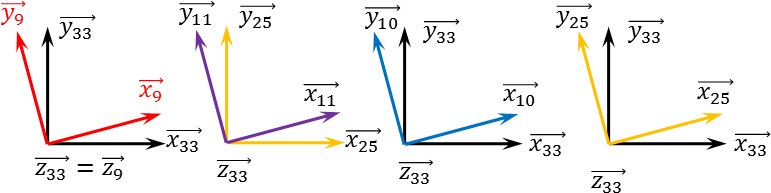
\includegraphics[width=.8\textwidth]{png/param}
\end{center}

\paragraph{}
\textit{Tracer le graphe des liaisons associé au train épicycloïdal.}
\begin{center}
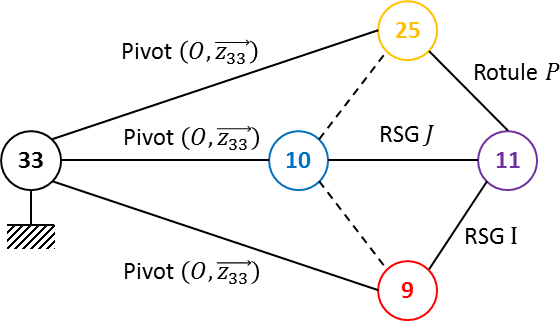
\includegraphics[width=.5\textwidth]{png/graphe}
\end{center}


\paragraph{}
\textit{Après avoir écrit la relation de roulement sans glissement entre \textbf{10} et \textbf{11}, décomposer le vecteur vitesse pour obtenir une relation entre : $R_{10}$, $R_{11}$, $\omega_{10/33}$, $\omega_{13/11}$ et $\omega_{13/33}$.}


D'après la relation de roulement sans glissement au point $J$, on a : 
$$
\vectv{J}{10}{11} = \vect{0} \quad \Longleftrightarrow \quad
\vectv{J}{10}{33}+\vectv{J}{33}{13}+\vectv{J}{13}{11} = \vect{0} 
$$

On a :
$$
\vectv{J}{10}{33} 
= \underbrace{\vectv{O}{10}{33}}_{\vect{0}} + \vect{JO}\wedge \vecto{10}{33} 
= -R_{10} \vect{x_{13}}\wedge \omega_{10/33}\vect{z_{33}}
=R_{10} \omega_{10/33}\vect{y_{33}}
$$

$$
\vectv{J}{13}{33} 
= \underbrace{\vectv{O}{13}{33}}_{\vect{0}} + \vect{JO}\wedge \vecto{13}{33} 
= -R_{10} \vect{x_{13}}\wedge \omega_{13/33}\vect{z_{33}}
=R_{10} \omega_{13/33}\vect{y_{33}}
$$

$$
\vectv{J}{13}{11} 
= \underbrace{\vectv{P}{13}{11}}_{\vect{0}} + \vect{JP}\wedge \vecto{13}{11} 
= -R_{11} \vect{x_{13}}\wedge \omega_{13/11}\vect{z_{33}}
=R_{11} \omega_{13/11}\vect{y_{33}}
$$

Au final, 

$$
\vectv{J}{10}{33}+\vectv{J}{33}{13}+\vectv{J}{13}{11} = \vect{0} 
\Longleftrightarrow
R_{10} \omega_{10/33}\vect{y_{33}} - R_{10} \omega_{13/33}\vect{y_{33}} +R_{11} \omega_{13/11}\vect{y_{33}}
= \vect{0} 
$$

$$
R_{10} \omega_{10/33}- R_{10} \omega_{13/33} +R_{11} \omega_{13/11}=0
$$



\paragraph{}
\textit{Après avoir écrit la relation de roulement sans glissement entre \textbf{11} et \textbf{9}, décomposer le vecteur vitesse pour obtenir une relation entre : $R_9$, $R_{11}$, $\omega_{9/33}$ et $\omega_{13/11}$ et $\omega_{13/33}$.}










D'après la relation de roulement sans glissement au point $I$, on a : 
$$
\vectv{I}{9}{11} = \vect{0} \quad \Longleftrightarrow \quad
\vectv{I}{9}{33}+\vectv{I}{33}{13}+\vectv{I}{13}{11} = \vect{0} 
$$

On a :
$$
\vectv{I}{9}{33} 
= \underbrace{\vectv{O}{9}{33}}_{\vect{0}} + \vect{IO}\wedge \vecto{9}{33} 
= -R_9 \vect{x_{13}}\wedge \omega_{9/33}\vect{z_{33}}
=R_9 \omega_{9/33}\vect{y_{33}}
$$

$$
\vectv{I}{13}{33} 
= \underbrace{\vectv{O}{13}{33}}_{\vect{0}} + \vect{IO}\wedge \vecto{13}{33} 
= -R_9 \vect{x_{13}}\wedge \omega_{13/33}\vect{z_{33}}
=R_9 \omega_{13/33}\vect{y_{33}}
$$

$$
\vectv{I}{13}{11} 
= \underbrace{\vectv{P}{13}{11}}_{\vect{0}} + \vect{IP}\wedge \vecto{13}{11} 
= R_{11} \vect{x_{13}}\wedge \omega_{13/11}\vect{z_{33}}
=-R_{11} \omega_{13/11}\vect{y_{33}}
$$

Au final, 

$$
\vectv{I}{9}{33}+\vectv{I}{33}{13}+\vectv{I}{13}{11} = \vect{0} 
\Longleftrightarrow
R_9 \omega_{9/33}\vect{y_{33}}-R_9 \omega_{13/33}\vect{y_{33}}-R_{11} \omega_{13/11}\vect{y_{33}} = \vect{0} 
$$

$$
R_9 \omega_{9/33}-R_9 \omega_{13/33}-R_{11} \omega_{13/11}=0
$$







\paragraph{}
\textit{Déterminer une relation géométrique permettant de lier $R_{9}$, $R_{11}$ et $R_{10}$.}

$$
R_{10}=R_9+2R_{11} \quad \quad R_{13}=R_9 + R_{11}
$$


\paragraph{}
\textit{A partir des 3 relations précédentes, montrer que : 
$$
\dfrac{5}{3}\omega_{(12/33)} = \omega_{(10/33)}+\omega_{(9/33)}
$$
On donne : $R_{10}=42\;mm$, $R_{9}=21\;mm$, $R_{11}=10,5 \;mm$.}

A partir des relations suivantes nous allons supprimer $\omega_{13/11}$ :
$$
\left\{
\begin{array}{l}
R_9 \omega_{9/33}-R_9 \omega_{13/33}-R_{11} \omega_{13/11}=0 \\
R_{10} \omega_{10/33}- R_{10} \omega_{13/33} +R_{11} \omega_{13/11}=0
\end{array}
\right.
$$

On a donc : 
$$
R_9 \omega_{9/33}-R_9 \omega_{13/33} = -R_{10} \omega_{10/33}+R_{10} \omega_{13/33}
\Longleftrightarrow
R_9 \omega_{9/33}-R_9 \omega_{13/33} -R_{10} \omega_{13/33}= -R_{10} \omega_{10/33}
$$


$$
\left( R_9 + R_{10}\right) \omega_{13/33} = R_9 \omega_{9/33}+R_{10}\omega_{10/33}
$$


\paragraph{}
\textit{Que se passe-t-il si le train avant est bloqué dans un obstacle ?}

Lors du blocage du train avant, $\omega_{9/33}=0$. En conséquence,  
$\dfrac{ R_9 + R_{10}}{ R_{10}} \omega_{13/33} =\omega_{10/33} \rightarrow 
\omega_{10/33} = 1,5 \cdot \omega_{13/33}$. Toute la puissance passe donc dans le train arrière.


\paragraph{}
\textit{Que se passe-t-il si le train arrière est bloqué dans un obstacle ?}

Dans ces conditions, $\omega_{10/33}=0$. En conséquence, 
$\omega_{9/33} = \dfrac{R_9 + R_{10}}{R_{10}} \omega_{13/33}  =1,5 \cdot \omega_{13/33}$.
Toute la puissance passe donc dans le train avant.

\paragraph{}
\textit{Que se passe-t-il si lorsque le différentiel est bloqué ?}

Dans ces conditions, $\omega_{9/33} =\omega_{13/33}$. En conséquence : 

$\left( R_9 + R_{10}\right) \omega_{13/33} = R_9 \omega_{13/33}+R_{10}\omega_{10/33}
\Longleftrightarrow
 R_{10} \omega_{13/33} =R_{10}\omega_{10/33}
\Longleftrightarrow
\omega_{13/33} =\omega_{10/33}
$

Ainsi, dans le cas où un train patinerait (sur la glace par exemple), si le différentiel n'est pas bloqué, le véhicule va s'enliser : toute la puissance passera dans le train qui patine et aucune puissance ne sera transmise dans le train qui accroche. En bloquant le différentiel, la puissance est équitablement répartie entre les trains. On peut ainsi déplacer le véhicule.

\newpage
\section{Arbre d'appui}
Les dessin de définition est coté en utilisant le système de tolérances générales suivant : \textbf{ISO 2768 mK}. Vous vous référerez au TD sur le kart pour connaître les intervalles de tolérance associés. 

\paragraph{}
\textit{En utilisant le dessin de définition, interprétez les spécifications géométriques suivantes :}

\begin{center}
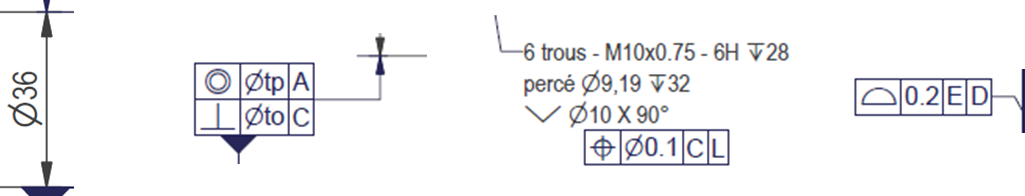
\includegraphics[width=.8\textwidth]{png/specif}
\end{center}
\end{document}
